\chapter{Options: Payoffs, No-Arbitrage Bounds, and Put--Call Parity}
\label{ch:options_payoffs}
\chaptermark{Options: payoffs and no-arb bounds}

You think Tesla might go up but are not sure, and do not want to
lose more than \$500 if wrong. How do you express that view? The
naive answer is ``buy a few shares and set a stop''. The options
answer is ``buy a call''. This chapter builds the call from first
principles: its payoff, its price bounds, and its relationship to
the put via the most famous identity in derivatives.

The treatment is pre--Black--Scholes. Nothing here requires a
stochastic differential equation, an Itô lemma, or a probability
measure. Every result is proved by writing down two portfolios,
comparing their payoffs in every state, and applying the
no-arbitrage axiom from \cref{ch:arbitrage_zoo}: if portfolio $A$
pays at least as much as $B$ in every state, $A$'s price today
is at least $B$'s. We need only the discount factor
$e^{-\rrf(\Tmat - t)}$ that converts a sure cash flow at maturity
into its time-$t$ value, plus algebra on $\max(x, 0)$. Volatility,
the central ingredient of \cref{ch:black_scholes}, does not appear
in this chapter.

\paragraph{Symbol anchor.} Throughout: $\Spx_t$ spot at time $t$;
$\Kstrike$ strike; $\Tmat$ maturity; $\rrf$ risk-free rate;
$\Call_t$ call price; $\Put_t$ put price; $\sigma$ volatility
(absent in this chapter).

\begin{backgroundbox}[Prerequisites]
From earlier in the book:
\begin{itemize}
  \item \Cref{ch:lob,ch:participants,ch:price_value}: exchanges,
  the limit order book, the bid--ask--mid--microprice family.
  Options trade on order books too; everything earlier about
  quoting, queues, and execution applies unchanged.
  \item \Cref{ch:arbitrage_zoo}, especially \S13.1's arbitrage
  template (\emph{state the observable, exhibit the portfolio,
  lock in the violation}). That chapter derived put--call parity
  once already in a diagnostic-arbitrage context with the worked
  example $\Spx = \Kstrike = 100$, $\rrf = 0.05$, $\Tmat = 1$
  giving $\Call - \Put \approx 4.877$. Here we re-derive it as
  the foundational replication identity: the
  \cref{ch:arbitrage_zoo} version asks ``how do you trade a
  parity violation?''; this one asks ``what does parity
  \emph{say} about how put and call relate?''
  \item Math: the expectation operator $\E[\cdot]$, continuous
  discounting $e^{-\rrf(\Tmat - t)}$, the indicator
  $\ind\{\Spx_T \geq \Kstrike\}$, and algebra on
  $\max(x, 0) = (x)^+$. No stochastic calculus.
\end{itemize}
\end{backgroundbox}

\section{Calls, puts, and payoffs}
\label{sec:ch14_payoffs}

An option is a contract whose value at a future date is a known
function of an \emph{underlying} asset's value at that date. The
simplest options, and the only ones in this chapter, are the
European call and put on a single non-dividend-paying stock.

Before the formula, the one-line mental model. A \emph{call}
with strike $\Kstrike = 100$ lets its holder buy the stock at
\$100 at expiry. If the stock ends at \$110, she exercises and
pockets \$10. If the stock ends at \$90, she walks away, losing
only whatever premium she paid up front. A \emph{put} is the
reverse: the right to \emph{sell} at the strike, valuable only
when the stock is below it. Both contracts floor losses at the
premium paid.

\begin{definition}[European call option]
\index{call option!European|textbf}\index{European call option|textbf}
\label{def:european_call}
A \emph{European call option} on an underlying asset $\Spx$, with
\emph{strike} $\Kstrike$ and \emph{maturity} (or \emph{expiry})
$\Tmat$, is a contract that grants its holder the \emph{right but
not the obligation} to buy one unit of $\Spx$ at price
$\Kstrike$ at time $\Tmat$. Its \emph{payoff} at expiry is
\begin{equation}
  \Call_T \;=\; \max(\Spx_T - \Kstrike,\, 0)
       \;\eqdef\; (\Spx_T - \Kstrike)^+,
  \label{eq:call_payoff}
\end{equation}
where $\Spx_T$ denotes the (random) value of the underlying at
time $\Tmat$. The option's price at any time $t < \Tmat$ is
written $\Call_t$ (or simply $\Call$ when the time is clear).
\end{definition}

The mechanics: at time $\Tmat$, if $\Spx_T > \Kstrike$ the holder
\emph{exercises} --- pays $\Kstrike$, takes delivery of an asset
worth $\Spx_T$, and immediately sells for $\Spx_T$, locking in
$\Spx_T - \Kstrike$. If $\Spx_T \leq \Kstrike$, exercise would be
a loss (paying $\Kstrike$ for something she could buy for
$\Spx_T$), so the contract grants the right to walk away. The
walking-away clause is the entire point: a forward obliges its
holder to transact at the strike with linear payoff
$\Spx_T - \Kstrike$ (potentially deeply negative); an option's
piecewise-linear payoff $(\Spx_T - \Kstrike)^+$ is non-negative
in every state.

\begin{definition}[European put option]
\index{put option!European|textbf}\index{European put option|textbf}
\label{def:european_put}
A \emph{European put option} on an underlying $\Spx$, with strike
$\Kstrike$ and maturity $\Tmat$, grants its holder the right but
not the obligation to \emph{sell} one unit of $\Spx$ at price
$\Kstrike$ at time $\Tmat$. Its payoff at expiry is
\begin{equation}
  \Put_T \;=\; \max(\Kstrike - \Spx_T,\, 0)
       \;=\; (\Kstrike - \Spx_T)^+.
  \label{eq:put_payoff}
\end{equation}
\end{definition}

A put is the reflection of a call across the strike. If
$\Spx_T < \Kstrike$ the put-holder exercises (buys at $\Spx_T$,
sells to the writer for $\Kstrike$, pockets $\Kstrike - \Spx_T$);
if $\Spx_T \geq \Kstrike$ she walks away.

Non-negativity of both payoffs is the source of every other
property below. Since $(\Spx_T - \Kstrike)^+$ and
$(\Kstrike - \Spx_T)^+$ are both $\geq 0$, no option price may be
negative; if it were, buying it would be a free positive payoff
plus a positive cash receipt at $t$ --- the simplest arbitrage.

\begin{definition}[American option]
\index{American option|textbf}
\label{def:american_option}
An \emph{American} call (or put) is identical to its European
counterpart except that the holder may exercise at \emph{any}
time $t \in [0, \Tmat]$, not only at expiry. American options
are the dominant exchange-traded variant on US equities; European
options dominate index and FX. The two coincide in payoff at
expiry but differ in the early-exercise option, which we treat
in \S\ref{sec:ch14_american}.
\end{definition}

The party who \emph{sells} an option is said to \emph{write} it.
A call writer is obligated to deliver the underlying at
$\Kstrike$ if the holder exercises; a put writer is obligated to
take delivery at $\Kstrike$. The writer's payoff is the negative
of the holder's:
\begin{equation*}
  \text{short call payoff} \;=\; -(\Spx_T - \Kstrike)^+,
  \qquad
  \text{short put payoff}  \;=\; -(\Kstrike - \Spx_T)^+,
\end{equation*}
both $\leq 0$. The writer can never make money at expiry from
the option alone, but she receives the \emph{premium} ($\Call_0$
or $\Put_0$) at $t = 0$ and hopes it exceeds the eventual payout.

\subsection{Moneyness}
\label{sec:ch14_moneyness}

Three pieces of jargon describe the relationship between spot
$\Spx_t$ and strike $\Kstrike$, used in every options conversation.

\begin{definition}[Moneyness]
\index{moneyness|textbf}
\label{def:moneyness}
A call option with strike $\Kstrike$ on underlying $\Spx_t$ is
called
\begin{itemize}
  \item \emph{in the money (ITM)} if $\Spx_t > \Kstrike$,
  \item \emph{at the money (ATM)} if $\Spx_t = \Kstrike$,
  \item \emph{out of the money (OTM)} if $\Spx_t < \Kstrike$.
\end{itemize}
A put option is called ITM if $\Spx_t < \Kstrike$, ATM if
$\Spx_t = \Kstrike$, and OTM if $\Spx_t > \Kstrike$. ``ITM''
always means \emph{exercising right now would yield a positive
payoff}; ``OTM'' means \emph{exercising right now would yield
zero payoff}; ``ATM'' is the borderline.
\end{definition}

Conventionally the strike is named: ``a 250-strike Tesla call''
means $\Kstrike = 250$. ``Buy me ATM Tesla calls'' means the
listed strike closest to current spot.

\subsection{Intrinsic value and time value}
\label{sec:ch14_intrinsic_time}

The price of an option before expiry is decomposed into two
non-negative parts.

\begin{definition}[Intrinsic and time value]
\index{intrinsic value|textbf}\index{time value (option)|textbf}
\label{def:intrinsic_time}
Let $\Call_t$ be the price of a European call on
non-dividend-paying $\Spx$ with strike $\Kstrike$ and maturity
$\Tmat \geq t$. Define
\begin{align}
  \text{intrinsic value} &\;\defeq\; (\Spx_t - \Kstrike)^+,
  \label{eq:intrinsic_call} \\
  \text{time value}      &\;\defeq\; \Call_t \;-\; (\Spx_t - \Kstrike)^+.
  \label{eq:time_value_call}
\end{align}
The same decomposition applies to a put with intrinsic value
$(\Kstrike - \Spx_t)^+$.
\end{definition}

Intrinsic value is what the option would pay if expiry were
\emph{now}. Time value is everything else --- the market's price
for the chance of going deeper in the money by $\Tmat$, plus the
carry effect of deferring the strike payment. We prove below
that time value is non-negative for European calls and peaks at
the money; for now it is just notation
$\Call_t = $ intrinsic $+$ time.

\subsection{Hockey-stick payoff diagrams}
\label{sec:ch14_hockey}

Traders call the piecewise-linear payoff curve a
\emph{hockey stick}. Plotting the four single-leg payoffs in the
$\Spx_T$--P\&L plane gives the visual grammar the rest of the
options material builds on.

\begin{figure}[htbp]
\centering
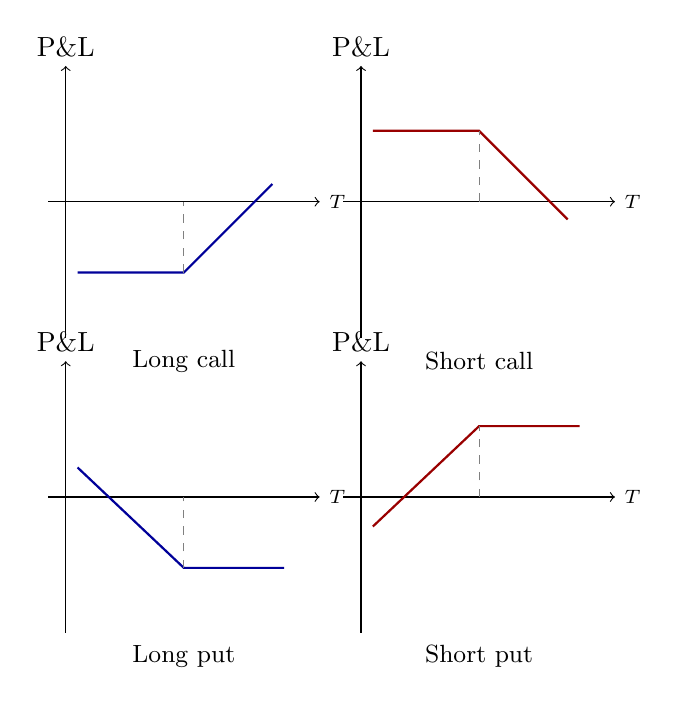
\begin{tikzpicture}[scale=0.75]
  % --- Long call ---
  \begin{scope}[xshift=0cm]
    \draw[->] (-0.3,0) -- (4.3,0) node[right]{$\Spx_T$};
    \draw[->] (0,-2.3) -- (0,2.3) node[above]{P\&L};
    \draw[thick, blue!60!black]
      (0.2,-1.2) -- (2,-1.2) -- (3.5,0.3);
    \draw[dashed, gray] (2,-1.2) -- (2,0) node[above, black, font=\tiny]{$\Kstrike$};
    \node at (2.0,-2.7) {\small Long call};
  \end{scope}
  % --- Short call ---
  \begin{scope}[xshift=5cm]
    \draw[->] (-0.3,0) -- (4.3,0) node[right]{$\Spx_T$};
    \draw[->] (0,-2.3) -- (0,2.3) node[above]{P\&L};
    \draw[thick, red!60!black]
      (0.2,1.2) -- (2,1.2) -- (3.5,-0.3);
    \draw[dashed, gray] (2,0) -- (2,1.2);
    \node[above, font=\tiny] at (2,0) {$\Kstrike$};
    \node at (2.0,-2.7) {\small Short call};
  \end{scope}
  % --- Long put ---
  \begin{scope}[xshift=0cm, yshift=-5cm]
    \draw[->] (-0.3,0) -- (4.3,0) node[right]{$\Spx_T$};
    \draw[->] (0,-2.3) -- (0,2.3) node[above]{P\&L};
    \draw[thick, blue!60!black]
      (0.2,0.5) -- (2,-1.2) -- (3.7,-1.2);
    \draw[dashed, gray] (2,-1.2) -- (2,0);
    \node[above, font=\tiny] at (2,0) {$\Kstrike$};
    \node at (2.0,-2.7) {\small Long put};
  \end{scope}
  % --- Short put ---
  \begin{scope}[xshift=5cm, yshift=-5cm]
    \draw[->] (-0.3,0) -- (4.3,0) node[right]{$\Spx_T$};
    \draw[->] (0,-2.3) -- (0,2.3) node[above]{P\&L};
    \draw[thick, red!60!black]
      (0.2,-0.5) -- (2,1.2) -- (3.7,1.2);
    \draw[dashed, gray] (2,0) -- (2,1.2);
    \node[above, font=\tiny] at (2,0) {$\Kstrike$};
    \node at (2.0,-2.7) {\small Short put};
  \end{scope}
\end{tikzpicture}
\caption{The four single-leg hockey-stick payoffs at expiry,
P\&L net of the premium paid or received at $t=0$. Long
positions are blue; short positions are red. The horizontal
asymptote of each curve is the premium with the appropriate
sign.}
\label{fig:hockey_sticks}
\end{figure}

Combining single legs gives \emph{spreads} and \emph{combinations}.
These reappear throughout \cref{ch:greeks_hedging,ch:vol_surface}.

\paragraph{Long call spread.} Long one call at $\Kstrike_1$,
short one at $\Kstrike_2 > \Kstrike_1$, same maturity. Payoff
$\min\bigl((\Spx_T - \Kstrike_1)^+,\, \Kstrike_2 - \Kstrike_1\bigr)$:
zero below $\Kstrike_1$, sloping up at $45^\circ$ in
$[\Kstrike_1, \Kstrike_2]$, capped at $\Kstrike_2 - \Kstrike_1$
above. Expresses ``prices rise, but modestly''.

\paragraph{Long put spread.} Long put at $\Kstrike_2$, short put
at $\Kstrike_1 < \Kstrike_2$. Capped at $\Kstrike_2 - \Kstrike_1$
above, zero below $\Kstrike_1$. Expresses ``prices fall, but
modestly'' --- the downside analogue of the call spread, and the
canonical cheap hedge against a bounded drawdown.

\paragraph{Long straddle and long strangle.} A \emph{straddle}
is a long call and long put at the same strike $\Kstrike$ and
maturity, payoff $|\Spx_T - \Kstrike|$. A \emph{strangle} uses
two strikes (call at $\Kstrike_2 > \Kstrike_1$, put at
$\Kstrike_1$); cheaper, but pays nothing in
$[\Kstrike_1, \Kstrike_2]$. Both express ``large move, either
direction'' --- a pure volatility bet, the topic of
\cref{ch:vol_surface}.

\subsection{Tesla worked example}
\label{sec:ch14_tesla}

Tesla trades at $\Spx_0 = \$240$. A 3-month European call with
strike $\Kstrike = \$250$ is quoted at premium $\Call_0 = \$12$.
Track the holder's P\&L in two expiry scenarios.

\paragraph{Scenario A: $\Spx_T = \$280$.} The call is ITM. The
holder exercises, paying $\$250$ for stock worth $\$280$:
\begin{equation*}
  \text{call payoff at expiry} \;=\; (280 - 250)^+ \;=\; \$30.
\end{equation*}
Subtract the \$12 premium paid at $t = 0$. \emph{Net P\&L = \$18.}

\paragraph{Scenario B: $\Spx_T = \$240$.} The call is OTM.
Exercising would mean paying \$250 for something worth \$240, so
the holder walks away:
\begin{equation*}
  \text{call payoff at expiry} \;=\; (240 - 250)^+ \;=\; \$0.
\end{equation*}
Subtract the \$12 premium. \emph{Net P\&L = $-\$12$.}

\paragraph{Break-even.} Net P\&L crosses zero when
$(\Spx_T - \Kstrike)^+ = \Call_0$, i.e.\
$\Spx_T = \Kstrike + \Call_0 = \$262$. Above \$262 the holder
makes money; in $[\$250, \$262]$ she exercises but loses some
premium; below \$250 she walks away and loses the full \$12.

The capped \$12 loss per share is the point of the contract: the
holder has converted ``buy 100 shares and pray'' into ``buy 100
calls, max loss \$1{,}200 regardless of crash''. That is the
answer to the chapter's opening question.

\begin{keyfactbox}[Option payoffs at expiry]
\label{kf:payoffs_expiry}
For a non-dividend-paying underlying $\Spx$:
\begin{align*}
  \text{long call:}  &\quad \Call_T = (\Spx_T - \Kstrike)^+, \\
  \text{long put:}   &\quad \Put_T  = (\Kstrike - \Spx_T)^+, \\
  \text{short call:} &\quad -(\Spx_T - \Kstrike)^+, \\
  \text{short put:}  &\quad -(\Kstrike - \Spx_T)^+.
\end{align*}
P\&L at expiry equals the payoff above minus the premium paid
(or plus the premium received). All four functions are piecewise
linear in $\Spx_T$ with a single kink at $\Spx_T = \Kstrike$.
\end{keyfactbox}

\begin{intuitionbox}
Takeaway: \emph{an option converts a linear view into a
piecewise-linear one.} A forward or stock position has slope
$\pm 1$ everywhere, symmetric P\&L, no downside cap without
selling. An option's payoff has slope $0$ on one side of the
strike and $\pm 1$ on the other. The kink is the entire content
of the contract: it is what the premium buys, and what the next
four chapters try to value.
\end{intuitionbox}

\section{No-arbitrage bounds by portfolio construction}
\label{sec:ch14_bounds}

Even before we can price options, no-arbitrage alone forces the
price into a tight interval. We prove five such bounds, each
following the same template.

\begin{keyfactbox}[The bound-by-replication template]
\label{kf:bound_template}
To prove ``price of $X$ at time $t$ is at least price of $Y$'',
construct portfolios $A$ and $B$ with $A_T \geq B_T$ in
\emph{every state}. By no-arbitrage, prices today satisfy
$\text{cost}_t(A) \geq \text{cost}_t(B)$; otherwise buying $A$
and selling $B$ at $t$ is a free lunch. For an equality, do it
in both directions, or show $A_T = B_T$ pointwise.
\end{keyfactbox}

We apply the template five times, with bounds increasing in
strength.

\subsection{Bound 1: a European call has non-negative price}
\label{sec:ch14_bound1}

\begin{proposition}
\label{prop:call_nonneg}
For any European call on a non-dividend-paying underlying, at
every $t \leq \Tmat$,
\begin{equation*}
  \Call_t \;\geq\; 0.
\end{equation*}
\end{proposition}

\begin{proof}
Let $A =$ ``one call'' and $B =$ ``nothing''. At maturity
$A_T = (\Spx_T - \Kstrike)^+ \geq 0 = B_T$, so
$\Call_t \geq 0$. Equivalently, if $\Call_t < 0$ the trader
receives $|\Call_t|$ for buying the call, holds to expiry,
collects the non-negative payoff, and makes money from nothing.
\end{proof}

By the same argument $\Put_t \geq 0$. This trivial bound matters
because every subsequent bound combines non-negativity with
discounting.

\subsection{Bound 2: a call costs no more than the underlying}
\label{sec:ch14_bound2}

\begin{proposition}
\label{prop:call_upper}
For any European call on a non-dividend-paying underlying, at
every $t \leq \Tmat$,
\begin{equation*}
  \Call_t \;\leq\; \Spx_t.
\end{equation*}
\end{proposition}

\begin{proof}
Let $A =$ ``one share'' and $B =$ ``one call''. At expiry
$A_T = \Spx_T$, $B_T = (\Spx_T - \Kstrike)^+$. In every state
$\Spx_T \geq (\Spx_T - \Kstrike)^+$: if $\Spx_T \geq \Kstrike$,
$\Spx_T \geq \Spx_T - \Kstrike$ since $\Kstrike \geq 0$; else
$\Spx_T \geq 0$ since the stock price is non-negative. So
$\Spx_t \geq \Call_t$.
\end{proof}

Economically: the most a call pays is $\Spx_T$ itself (achieved
as $\Kstrike \to 0$, where the call \emph{is} the stock), so
paying more than $\Spx_t$ for the right to buy at $\Kstrike$ is
worse than buying the stock outright.

\subsection{Bound 3: the European call lower bound}
\label{sec:ch14_bound3}

This is the central bound. Sharper than intrinsic value (because
it discounts the strike), it proves European call $=$ American
call on non-dividend stock in \S\ref{sec:ch14_american}.

\begin{theorem}[European call lower bound]
\label{thm:call_lower_bound}
For any European call on a non-dividend-paying underlying at
risk-free rate $\rrf$, at every $t \leq \Tmat$,
\begin{equation}
  \Call_t \;\geq\; \max\!\bigl(\Spx_t - \Kstrike\,e^{-\rrf(\Tmat - t)},\;\, 0\bigr).
  \label{eq:call_lower_bound}
\end{equation}
\end{theorem}

\begin{proof}
The non-negativity half is \cref{prop:call_nonneg}. For the other
half, define two portfolios:
\begin{itemize}
  \item \textbf{Portfolio A:} long one call (cost $\Call_t$) plus
  long a riskless zero-coupon bond paying $\Kstrike$ at time
  $\Tmat$ (cost $\Kstrike e^{-\rrf(\Tmat-t)}$). Total cost at
  $t$:
  \begin{equation*}
    \text{cost}_t(A) \;=\; \Call_t \;+\; \Kstrike e^{-\rrf(\Tmat - t)}.
  \end{equation*}
  \item \textbf{Portfolio B:} long one share of $\Spx$. Cost at
  $t$: $\Spx_t$.
\end{itemize}
At maturity:
\begin{align*}
  A_T \;&=\; (\Spx_T - \Kstrike)^+ \;+\; \Kstrike
        \;=\; \max\!\bigl(\Spx_T - \Kstrike + \Kstrike,\; 0 + \Kstrike\bigr)
        \;=\; \max(\Spx_T,\, \Kstrike), \\
  B_T \;&=\; \Spx_T.
\end{align*}
Since $\max(\Spx_T, \Kstrike) \geq \Spx_T$ in every state, we
have $A_T \geq B_T$ everywhere. By the template,
\begin{equation*}
  \Call_t \;+\; \Kstrike e^{-\rrf(\Tmat - t)} \;\geq\; \Spx_t,
\end{equation*}
which rearranges to
$\Call_t \geq \Spx_t - \Kstrike e^{-\rrf(\Tmat - t)}$. Combined
with \cref{prop:call_nonneg}, this is precisely
\eqref{eq:call_lower_bound}.
\end{proof}

The bound strictly exceeds intrinsic value $(\Spx_t - \Kstrike)^+$
whenever $\rrf > 0$ and $t < \Tmat$, since
$\Kstrike e^{-\rrf(\Tmat - t)} < \Kstrike$. The discounted
strike is a pure deterministic carry effect: even on a constant
stock with zero volatility, an ATM call costs at least
$\Spx_t(1 - e^{-\rrf(\Tmat-t)})$, because the holder defers
paying $\Kstrike$ to $\Tmat$ rather than paying $\Spx_t$ now.
Volatility makes the actual price exceed the bound; the bound
itself is volatility-free.

\subsection{Worked example: the lower bound at $\Spx = \Kstrike = 100$}
\label{sec:ch14_lower_example}

Take $\Spx_t = \$100$, $\Kstrike = \$100$, $\rrf = 5\%$,
$\Tmat - t = 1$ year. The discounted strike is
\begin{equation*}
  \Kstrike e^{-\rrf(\Tmat - t)}
  \;=\; 100 \cdot e^{-0.05}
  \;\approx\; 95.1229,
\end{equation*}
so the lower bound is
\begin{equation*}
  \max(\Spx_t - \Kstrike e^{-\rrf(\Tmat - t)},\, 0)
  \;=\; 100\bigl(1 - e^{-0.05}\bigr)
  \;\approx\; \$4.8771.
\end{equation*}
The option is ATM with zero intrinsic value, yet no-arb forces
price above \$4.8771. A market quoting below this lets a trader
buy the call, buy a one-year bond paying \$100, short one share,
and lock in positive cash today with non-negative cash at expiry.
The same number reappears in the parity example: at
$\Spx = \Kstrike$ both the ATM call lower bound and the parity
RHS equal $100(1 - e^{-0.05}) \approx 4.877$.

\subsection{Bound 4: the European put lower bound}
\label{sec:ch14_bound4}

Mirror image of the call bound; proof identical with $A$, $B$
swapped.

\begin{proposition}[European put lower bound]
\label{prop:put_lower_bound}
For any European put on a non-dividend-paying underlying,
\begin{equation}
  \Put_t \;\geq\; \max\!\bigl(\Kstrike e^{-\rrf(\Tmat - t)} - \Spx_t,\;\, 0\bigr).
  \label{eq:put_lower_bound}
\end{equation}
\end{proposition}

\begin{proof}
Non-negativity follows as in \cref{prop:call_nonneg}. For the
discount-aware half, set
\begin{itemize}
  \item \textbf{Portfolio A:} long one put plus long one share.
  Cost at $t$: $\Put_t + \Spx_t$.
  \item \textbf{Portfolio B:} long a zero-coupon bond paying
  $\Kstrike$ at $\Tmat$. Cost at $t$:
  $\Kstrike e^{-\rrf(\Tmat-t)}$.
\end{itemize}
At maturity, $A_T = (\Kstrike - \Spx_T)^+ + \Spx_T =
\max(\Kstrike, \Spx_T) \geq \Kstrike = B_T$ in every state. By
the template, $\Put_t + \Spx_t \geq \Kstrike e^{-\rrf(\Tmat-t)}$,
which rearranges to
$\Put_t \geq \Kstrike e^{-\rrf(\Tmat-t)} - \Spx_t$. Combined
with $\Put_t \geq 0$, this is \eqref{eq:put_lower_bound}.
\end{proof}

\subsection{Bound 5: the European put upper bound}
\label{sec:ch14_bound5}

\begin{proposition}[European put upper bound]
\label{prop:put_upper_bound}
For any European put on a non-dividend-paying underlying,
\begin{equation}
  \Put_t \;\leq\; \Kstrike e^{-\rrf(\Tmat - t)}.
  \label{eq:put_upper_bound}
\end{equation}
\end{proposition}

\begin{proof}
At maturity the put pays at most $\Kstrike$, achieved when
$\Spx_T = 0$. Let $A$ be a zero-coupon bond paying $\Kstrike$
at $\Tmat$ (cost $\Kstrike e^{-\rrf(\Tmat-t)}$) and $B$ be a
European put. Then $A_T = \Kstrike \geq (\Kstrike - \Spx_T)^+ =
B_T$ in every state, since the right-hand side is at most
$\Kstrike$. By the template, $\Kstrike e^{-\rrf(\Tmat-t)}
\geq \Put_t$.
\end{proof}

The upper-bound asymmetry --- call bounded by $\Spx_t$, put by
$\Kstrike e^{-\rrf(\Tmat-t)}$ --- reflects that the call is
unbounded above ($\Spx_T$ has no ceiling) while the put is
bounded above at $\Kstrike$ (the underlying cannot fall below
zero).

\begin{keyfactbox}[European option price bounds (no dividends)]
\label{kf:option_bounds}
For a European call $\Call_t$ and European put $\Put_t$ on a
non-dividend-paying underlying $\Spx$ with strike $\Kstrike$,
maturity $\Tmat$, and risk-free rate $\rrf$, the following
hold at every $t \leq \Tmat$:
\begin{align}
  \max\!\bigl(\Spx_t - \Kstrike e^{-\rrf(\Tmat-t)},\, 0\bigr)
    &\;\leq\; \Call_t \;\leq\; \Spx_t,
    \label{eq:call_band} \\[4pt]
  \max\!\bigl(\Kstrike e^{-\rrf(\Tmat-t)} - \Spx_t,\, 0\bigr)
    &\;\leq\; \Put_t \;\leq\; \Kstrike e^{-\rrf(\Tmat-t)}.
    \label{eq:put_band}
\end{align}
Proved by explicit two-portfolio construction. Holds without any
assumption on the distribution of $\Spx_T$, volatility, or the
existence of any pricing model
\citep{damodaranOptionsArbitrage}.
\end{keyfactbox}

\begin{intuitionbox}
\Cref{eq:call_band,eq:put_band} pin the option to an interval
depending only on $\Spx_t$, $\Kstrike$, $\rrf$, $\Tmat - t$. The
discount factor $e^{-\rrf(\Tmat - t)}$ is the \emph{only}
time-value ingredient: no volatility, drift, or probability
measure --- none was needed. Volatility is what
\cref{ch:black_scholes} adds: it picks a specific point inside
the band. Black--Scholes is geometrically a rule for selecting
that precise location.
\end{intuitionbox}

\section{Put--call parity}
\label{sec:ch14_parity}

The previous section pinned each option to an interval.
Put--call parity is sharper: an \emph{equality} ties call and
put, leaving three degrees of freedom in
$\{\Call_t, \Put_t, \Spx_t, \Kstrike e^{-\rrf(\Tmat-t)}\}$.
\Cref{ch:arbitrage_zoo} stated the identity in the diagnostic
context. Here we re-derive it in the options-theory context:
the four contracts can be assembled into a basket that \emph{is}
a long stock position, so basket and stock share the same price.

\subsection{The replicating portfolio}
\label{sec:ch14_parity_setup}

The intuition before the algebra: a long call plus the
discounted strike in the bank has the same expiry payoff as a
long put plus one share --- both baskets deliver
$\max(\Spx_T, \Kstrike)$ in every state. Two portfolios with
identical payoffs in every state must cost the same today, or
buying the cheaper and shorting the dearer is a free lunch.
That equality \emph{is} put--call parity.

Engineer a portfolio whose payoff is exactly $\Spx_T$ in every
state using a call, a put, and a bond. Define
\begin{equation}
  V_t \;\defeq\; \Call_t \;-\; \Put_t \;+\; \Kstrike e^{-\rrf(\Tmat - t)}.
  \label{eq:Vt_definition}
\end{equation}
$V_t$ is the cost of buying one call, selling one put (a short
put is an inflow $\Put_t$, hence the minus sign), and buying a
bond paying $\Kstrike$ at $\Tmat$. We claim $V_T = \Spx_T$ in
every state and prove by two cases.

\begin{theorem}[Put--call parity]
\label{thm:put_call_parity}
For a European call $\Call$ and European put $\Put$ on the same
non-dividend-paying underlying $\Spx$ with the same strike
$\Kstrike$ and same maturity $\Tmat$, at risk-free rate $\rrf$,
\begin{equation}
  \Call_t \;-\; \Put_t \;=\; \Spx_t \;-\; \Kstrike e^{-\rrf(\Tmat - t)}
  \qquad \text{for every } t \leq \Tmat.
  \label{eq:put_call_parity_ch14}
\end{equation}
\end{theorem}

\begin{proof}
Let $V_t$ be the portfolio of \eqref{eq:Vt_definition}. Compute
$V_T$ in two cases.

\textbf{Case 1: $\Spx_T \geq \Kstrike$.} Call is ITM, pays
$\Spx_T - \Kstrike$. Short put is OTM, pays $0$. Bond pays
$\Kstrike$:
\begin{equation*}
  V_T \;=\; (\Spx_T - \Kstrike) \;-\; 0 \;+\; \Kstrike
        \;=\; \Spx_T.
\end{equation*}

\textbf{Case 2: $\Spx_T < \Kstrike$.} Call is OTM, pays $0$.
Short put is ITM; we owe $\Kstrike - \Spx_T$. Bond pays
$\Kstrike$:
\begin{equation*}
  V_T \;=\; 0 \;-\; (\Kstrike - \Spx_T) \;+\; \Kstrike
        \;=\; \Spx_T.
\end{equation*}

In both cases $V_T = \Spx_T$. So $V$ matches one share
pointwise; by the equality corner of the template,
$V_t = \Spx_t$ at every $t$:
\begin{equation*}
  \Call_t \;-\; \Put_t \;+\; \Kstrike e^{-\rrf(\Tmat - t)}
  \;=\; \Spx_t,
\end{equation*}
which is \eqref{eq:put_call_parity_ch14}.
\end{proof}

\subsection{Synthetic positions}
\label{sec:ch14_synthetics}

Rearranging \eqref{eq:put_call_parity_ch14} gives the four
\emph{synthetic} relations every options trader has memorised:
\begin{align}
  \text{long stock}        \;&\equiv\;
    \text{long call} \;+\; \text{short put} \;+\;
    \text{long bond of notional } \Kstrike e^{-\rrf(\Tmat-t)},
    \label{eq:synth_stock} \\
  \text{long call}        \;&\equiv\;
    \text{long put} \;+\; \text{long stock} \;-\;
    \text{long bond of notional } \Kstrike e^{-\rrf(\Tmat-t)},
    \label{eq:synth_call} \\
  \text{long put}         \;&\equiv\;
    \text{long call} \;-\; \text{long stock} \;+\;
    \text{long bond of notional } \Kstrike e^{-\rrf(\Tmat-t)},
    \label{eq:synth_put} \\
  \text{long bond}        \;&\equiv\;
    \text{long stock} \;-\; \text{long call} \;+\; \text{long put}.
    \label{eq:synth_bond}
\end{align}
These are pointwise identities, not approximations.
\Cref{eq:synth_stock} is the ``conservation law'' form: long
stock equals the long-call / short-put / bond combination.
\Cref{eq:synth_call} is how a market maker short a put (a client
sold to her) manufactures the equivalent long call: buy the
underlying, borrow the discounted strike.
\Cref{ch:arbitrage_zoo} showed how to trade a parity violation;
\eqref{eq:synth_stock}--\eqref{eq:synth_bond} are the same
identity rearranged for desk use.

\begin{keyfactbox}[Put--call parity]
\label{kf:put_call_parity_ch14}
For European call and put with the same strike $\Kstrike$ and
maturity $\Tmat$ on a non-dividend-paying underlying at
risk-free rate $\rrf$,
\begin{equation*}
  \boxed{\;\Call_t \;-\; \Put_t \;=\; \Spx_t \;-\; \Kstrike e^{-\rrf(\Tmat - t)}\;}
\end{equation*}
holds at every $t \leq \Tmat$, by no-arbitrage, with no
distributional assumption on $\Spx$. The four-asset relation
has three degrees of freedom: knowing any three of
$\{\Call, \Put, \Spx, \Kstrike e^{-\rrf(\Tmat-t)}\}$ determines
the fourth.
\end{keyfactbox}

\subsection{Worked numerical example}
\label{sec:ch14_parity_example}

Same parameters as before. The parity RHS is
\begin{equation*}
  \Spx_t - \Kstrike e^{-\rrf(\Tmat - t)}
    \;=\; 100\,(1 - e^{-0.05})
    \;\approx\; 4.8771,
\end{equation*}
so any European call/put pair here must satisfy
$\Call - \Put \approx 4.8771$. The same \$4.877 was the ATM
lower bound in \S\ref{sec:ch14_lower_example} and the parity
RHS in \cref{ch:arbitrage_zoo}: at $\Spx = \Kstrike$ those
quantities coincide.

If the market quotes $\Call = \$8$, parity forces
\begin{equation*}
  \Put \;=\; \Call - \bigl(\Spx_t - \Kstrike e^{-\rrf(\Tmat - t)}\bigr)
       \;=\; 8 - 4.8771
       \;\approx\; \$3.1229.
\end{equation*}
A market quoting call at \$8 and put at \$2 is inconsistent: by
\cref{ch:arbitrage_zoo} \S13.4 the trader sells the call at \$8,
buys the put at \$2, buys the stock at \$100, borrows
$100 e^{-0.05} \approx \$95.1229$, locking in net inflow
$8 - 2 - 100 + 95.1229 \approx \$1.1229$ against zero liability
at expiry. Inflow exactly equals the parity violation
$|(8-2) - 4.8771| = \$1.1229$. \Cref{ch:arbitrage_zoo} discusses
why such violations rarely appear on liquid exchanges; parity's
content here is that it pins the put price given the call.

\begin{intuitionbox}
Put--call parity is derivatives' conservation law. Four
quantities (call, put, spot, discounted strike) related by one
identity, leaving three degrees of freedom. Any consistent
options model must respect it --- Black--Scholes, Heston, a
neural network trained on chain data. Parity does not tell you
what the call is worth (no more than $E = mc^2$ tells you the
energy of a specific system); it tells you what the call is
worth \emph{relative to} the put, halving the problem.
\end{intuitionbox}

\begin{pitfallbox}[Parity breaks with discrete dividends]
\label{pf:parity_dividends_ch14}
The clean form $\Call_t - \Put_t = \Spx_t - \Kstrike e^{-\rrf(\Tmat-t)}$
assumes no dividends between $t$ and $\Tmat$. Real equities pay
dividends on discrete ex-div dates, and the dividend goes to
whoever holds the \emph{share} on that date, not to the
synthetic-stock holder. The corrected parity for dividend PV
$PV(D)$ between $t$ and $\Tmat$ is
\begin{equation}
  \Call_t \;-\; \Put_t \;=\; \Spx_t \;-\; PV(D) \;-\; \Kstrike e^{-\rrf(\Tmat - t)}.
  \label{eq:parity_dividends}
\end{equation}
Derivation is identical to \cref{thm:put_call_parity}, except
portfolio $V$ now pays out $PV(D)$ in dividends along the way;
the synthetic stock must be cheaper than cash stock by $PV(D)$
today. Forgetting $PV(D)$ is the most common failure mode of
parity scanners on dividend-paying single names \citeHull{}
(Ch~$10$). Same correction appears in the cost-of-carry formula
of \cref{ch:arbitrage_zoo}, for the same reason: synthetic stock
does not receive the dividend stream.
\end{pitfallbox}

\section{American options and early exercise}
\label{sec:ch14_american}

An American call grants strictly more rights than European
(exercise anywhere in $[0, \Tmat]$, not just at $\Tmat$), and a
richer contract should command a higher price. The theorem of
this section: on a non-dividend-paying stock the American and
European call prices are \emph{equal}. The early-exercise right
on a call has zero economic value when there are no dividends.

\subsection{The theorem and its proof}
\label{sec:ch14_amer_proof}

\begin{theorem}[American call $=$ European call, no dividends]
\label{thm:american_eq_european}
Let $\Call^{\mathrm{Am}}_t$ and $\Call^{\mathrm{Eu}}_t$ denote
the prices at time $t$ of an American and a European call
respectively, both on the same non-dividend-paying underlying
$\Spx$ with the same strike $\Kstrike$ and maturity $\Tmat$, at
risk-free rate $\rrf > 0$. Then
\begin{equation*}
  \Call^{\mathrm{Am}}_t \;=\; \Call^{\mathrm{Eu}}_t
  \quad\text{for every } t \in [0, \Tmat].
\end{equation*}
\end{theorem}

\begin{proof}
We prove the equality in three steps.

\textbf{Step 1: $\Call^{\mathrm{Am}}_t \geq \Call^{\mathrm{Eu}}_t$.}
The American grants every European right plus early exercise.
A contract with more rights cannot sell for less; otherwise buy
the American, sell the European, pocket the difference, and hold
both to expiry (the American replicates the European exercise).

\textbf{Step 2: European lower bound exceeds intrinsic value.}
\Cref{thm:call_lower_bound} gives
\begin{equation*}
  \Call^{\mathrm{Eu}}_t \;\geq\;
    \max\!\bigl(\Spx_t - \Kstrike e^{-\rrf(\Tmat - t)},\; 0\bigr).
\end{equation*}
For $t < \Tmat$ with $\rrf > 0$, $\Kstrike e^{-\rrf(\Tmat-t)} <
\Kstrike$, so
\begin{equation*}
  \Spx_t - \Kstrike e^{-\rrf(\Tmat - t)}
  \;>\; \Spx_t - \Kstrike.
\end{equation*}
Whenever the RHS is non-negative, the European call exceeds its
intrinsic value. (When intrinsic is zero, $\Call^{\mathrm{Eu}}_t
\geq 0$ already gives the result; we only need strictness ITM.)

\textbf{Step 3: early exercise is strictly worse than selling.}
An American holder considering exercise at $t < \Tmat$ replaces
the option with intrinsic value $\Spx_t - \Kstrike$. But selling
fetches $\Call^{\mathrm{Am}}_t$, and by Steps 1--2,
\begin{equation*}
  \Call^{\mathrm{Am}}_t \;\geq\; \Call^{\mathrm{Eu}}_t
       \;>\; \Spx_t - \Kstrike,
\end{equation*}
so selling dominates exercising. A rational holder never
early-exercises.

\textbf{Conclusion.} With no early exercise, American and
European exercise policies match (both at $\Tmat$), payoffs at
$\Tmat$ match, so by the equality corner of the template
$\Call^{\mathrm{Am}}_t = \Call^{\mathrm{Eu}}_t$.
\end{proof}

\begin{keyfactbox}[American call on non-dividend stock]
\label{kf:american_call}
For a call on non-dividend underlying at $\rrf > 0$, American
$=$ European; early exercise has zero economic value. The only
major derivatives-pricing theorem that requires no model: it
follows from the European-call lower bound alone
\citep{merton1973rational}.
\end{keyfactbox}

\subsection{Why the put is different}
\label{sec:ch14_amer_put}

The American put is different. Replaying Step 2 with put bounds
gives $\Put^{\mathrm{Eu}}_t \geq \Kstrike e^{-\rrf(\Tmat-t)} -
\Spx_t$, which is \emph{less} than intrinsic
$\Kstrike - \Spx_t$ when $\rrf > 0$ (discounting shrinks the
bound). Step 3 breaks: deep-ITM put intrinsic can exceed the
European price, so an American holder sometimes exercises
early. Intuition: early-exercising a put accelerates receipt of
$\Kstrike$ in cash (positive carry at $\rrf > 0$);
early-exercising a call accelerates the \emph{payment} of
$\Kstrike$ (negative carry). Calls and puts are asymmetric
under early exercise because cash and stock are asymmetric
under positive rates.

Characterising the American-put exercise boundary requires
binomial or PDE valuation; see \cref{ch:numerical_methods}. The
chapter-level fact: American calls on non-dividend stock $=$
European; American puts can be worth strictly more.

\subsection{Dividends re-enable early exercise on calls}
\label{sec:ch14_amer_div}

\Cref{thm:american_eq_european} requires no dividends. With a
discrete dividend $D$ on ex-date $t_D \in (t, \Tmat)$, holding
the share beats holding the call by $D$ on $t_D$. Just before
$t_D$, an American call holder faces: exercise and capture $D$,
or hold and keep time value. Exercise is optimal when $D$
exceeds the time value about to be lost. This is the only
situation where early exercise of an American call is rational,
and it is why on US single names American-call exercise
clusters a day or two before ex-div dates \citeHull{}
(Ch~$15$).

\begin{intuitionbox}
Early-exercising a call trades time value for intrinsic. On
non-dividend stock, time value is strictly positive (the
European lower bound proves it), so the trade is strictly bad.
Dividends create an inflow the call-holder forgoes; a large
enough dividend overpays for time value, and exercise becomes
rational. The American-put case trades time value for early
receipt of $\Kstrike$, which earns interest and can dominate.
Cash and stock are asymmetric under $\rrf > 0$ --- that is the
entire content of early exercise.
\end{intuitionbox}

\begin{historybox}
The observation that long call $+$ short put behaves like long
stock dates back to Russell Sage's synthetic-loan trades on the
New York exchanges in the $1860$s. The first formal statement
in academic finance is Stoll \citep{hostoll1981} ($1969$, with
a $1981$ follow-up cited here for the print version). The
rigorous arbitrage proof and the American-$=$-European theorem
are due to Merton's $1973$ Bell Journal paper
\citep{merton1973rational}, companion to Black--Scholes.
Merton's paper is unusual for being almost entirely model-free:
its results are no-arb inequalities like those here, and remain
true under any model.
\end{historybox}

\section{Applications and synthesis}
\label{sec:ch14_apps}

\begin{prosperitybox}
The Round 3--4 \texttt{VOLCANIC\_ROCK\_VOUCHERS} of IMC
Prosperity 3 were synthetic European calls on
\texttt{VOLCANIC\_ROCK}, five strikes
$\{9500, 9750, 10000, 10250, 10500\}$, single expiry;
\texttt{VOLCANIC\_ROCK} traded near 10{,}000 seashells (see
\texttt{imc-prosperity-3/README.md}). Voucher payoff was
$(\Spx_T - \Kstrike)^+$ in seashells, traded on the standard
order book, so all no-arb bounds here applied. Top teams
exploited the structure two ways:
\begin{itemize}
  \item \textbf{Bound enforcement.} Whenever a voucher quoted
  below $\max(\Spx - \Kstrike e^{-\rrf(\Tmat-t)}, 0)$: long
  voucher, long bond, short underlying. With Prosperity's
  rate at zero and short maturity the bound collapsed to
  intrinsic value, but the enforcement instinct was the same.
  \item \textbf{Cross-strike consistency.} The relative-value
  bounds of \cref{ch:arbitrage_zoo} (lower-strike calls
  $\geq$ higher-strike) and the convexity bound gave a
  second family of arbitrages when the five strikes drifted.
\end{itemize}
\Cref{ch:black_scholes} adds the vol-aware Black--Scholes
machinery that top teams actually used to quote and hedge (not
just police bounds); \cref{ch:greeks_hedging,ch:vol_surface}
finish the toolkit. The bounds here are the correctness floor
below which any voucher model is demonstrably wrong.
\end{prosperitybox}

\begin{gsbox}
On a Goldman equity-derivatives desk, the first sanity check a
Strat runs against a listed options book is put--call parity.
The pricing system computes, per (strike, maturity) cell,
\begin{equation*}
  \mathrm{LHS} \;=\; \Call_t - \Put_t,
  \qquad
  \mathrm{RHS} \;=\; \Spx_t - PV(D) - \Kstrike e^{-\rrf(\Tmat-t)},
\end{equation*}
and flags cells where $|\mathrm{LHS} - \mathrm{RHS}|$ exceeds
the bid--ask width plus estimated borrow cost. A real flag is
rare and matters: stale quote, unprocessed corporate action,
or --- rarest --- a capturable arb. Most flags resolve to three
causes: hard-to-borrow names (missing $-y$ borrow term),
unscheduled corporate actions (spin-offs, specials), or
low-liquidity maturities where the spread is wider than the
apparent violation. The Strat's job is not to trade the gap
(vol traders do that) but to \emph{maintain the flagging
model}, and to explain to the trader within minutes whether a
flag is real or noise. Memorising parity as
$\Call - \Put = \Spx - PV(D) - \Kstrike e^{-\rrf \Tmat}$ is a
Day-1 desk requirement.
\end{gsbox}

\section{Key facts to memorise}
\label{sec:ch14_keyfacts}

\begin{itemize}
  \item A \emph{European call} pays $(\Spx_T - \Kstrike)^+$ at
  expiry. A \emph{European put} pays $(\Kstrike - \Spx_T)^+$.
  Both payoffs are non-negative, so option prices are
  non-negative.
  \item ITM means exercising right now would give a positive
  payoff; OTM means it would give zero; ATM is the borderline.
  The intrinsic--time-value decomposition writes
  $\Call_t = (\Spx_t - \Kstrike)^+ + (\text{time value})$, with
  time value $\geq 0$ for European calls.
  \item European call bounds (no dividends):
  $\max(\Spx_t - \Kstrike e^{-\rrf(\Tmat-t)},\, 0) \leq \Call_t
  \leq \Spx_t$.
  \item European put bounds:
  $\max(\Kstrike e^{-\rrf(\Tmat-t)} - \Spx_t,\, 0) \leq \Put_t
  \leq \Kstrike e^{-\rrf(\Tmat-t)}$.
  \item Every bound is proved by writing down two portfolios and
  comparing payoffs in every state. No distributional or
  volatility assumption is needed.
  \item \textbf{Put--call parity} (no dividends):
  $\Call_t - \Put_t = \Spx_t - \Kstrike e^{-\rrf(\Tmat-t)}$,
  exact, model-free, by no-arbitrage.
  \item Worked sanity check: $\Spx = \Kstrike = 100$,
  $\rrf = 5\%$, $\Tmat = 1$ gives $\Call - \Put \approx 4.877$
  and an at-the-money lower bound of the same $\approx 4.877$.
  \item Synthetic relations: long stock $\equiv$ long call $+$
  short put $+$ long bond; long call $\equiv$ long put $+$
  long stock $-$ long bond; long put $\equiv$ long call $-$
  long stock $+$ long bond.
  \item With discrete dividends $PV(D)$:
  $\Call_t - \Put_t = \Spx_t - PV(D) - \Kstrike e^{-\rrf(\Tmat-t)}$.
  Forgetting $PV(D)$ is the canonical false-positive of a
  parity scanner.
  \item \textbf{American $=$ European call} on a
  non-dividend-paying stock at $\rrf > 0$. The proof uses only
  the European-call lower bound: selling the option is always
  strictly better than exercising it.
  \item American \emph{puts} can be optimal to early-exercise;
  dividends re-enable early exercise on American calls just
  before ex-dividend dates. Forward-reference
  \cref{ch:numerical_methods} for the algorithmic exercise
  boundary.
  \item Volatility plays no role in any result of this chapter.
  Volatility appears in \cref{ch:black_scholes}, where it picks
  a specific point inside the no-arb interval carved out by the
  bounds above.
\end{itemize}
